\documentclass[11pt]{article}
\usepackage{amsmath}
\usepackage[sc]{mathpazo} %Like Palatino with extensive math support
\usepackage{fullpage}
%\usepackage[authoryear,sectionbib,sort]{natbib}
\usepackage[square,sort,comma,numbers]{natbib}
\linespread{1.7}
\usepackage[utf8]{inputenc}
\usepackage{lineno}
\usepackage{titlesec}
\usepackage{xcolor}
\newcommand{\tom}[2]{{\color{red}{#1}}\footnote{\textit{\color{red}{#2}}}} 
\newcommand{\ali}[2]{{\color{blue}{#1}}\footnote{\textit{\color{blue}{#2}}}}  


\titleformat{\section}[block]{\Large\bfseries\filcenter}{\thesection}{1em}{}
\titleformat{\subsection}[block]{\Large\itshape\filcenter}{\thesubsection}{1em}{}
\titleformat{\subsubsection}[block]{\large\itshape}{\thesubsubsection}{1em}{}
\titleformat{\paragraph}[runin]{\itshape}{\theparagraph}{1em}{}[.]\renewcommand{\refname}{Literature Cited}


%%%%%%%%%%%%%%%%%%%%%
% Line numbering
%%%%%%%%%%%%%%%%%%%%%
%
% Please use line numbering with your initial submission and
% subsequent revisions. After acceptance, please turn line numbering
% off by adding percent signs to the lines %\usepackage{lineno} and
% to %\linenumbers{} and %\modulolinenumbers[3] below.
%
% To avoid line numbering being thrown off around math environments,
% the math environments have to be wrapped using
% \begin{linenomath*} and \end{linenomath*}
%
% (Thanks to Vlastimil Krivan for pointing this out to us!)

\title{Thank you, next: partner turnover elevates benefits of mutualism for an ant-tended plant}


\author{Alexandra Campbell$^{1,\ast}$ \\ 
	Tom E.X. Miller$^{1}$}

\date{}

\begin{document}
	
	\maketitle
	
	\noindent{} 1. Program in Ecology and Evolutionary Biology, Department of BioSciences, Rice University, Houston, Texas 77005;
	
	\noindent{} $\ast$ Corresponding author; e-mail: amc49@rice.edu.
	
	
	\textit{Manuscript elements}: 
	
	\bigskip
	
	\textit{Keywords}: 
	
	\bigskip
	
	\textit{Manuscript type}: Article.
	
	\bigskip
	
	\noindent{\footnotesize Prepared using the suggested \LaTeX{} template for \textit{Am.\ Nat.}}
	
\linenumbers{}
\modulolinenumbers[3]

\newpage{}

\section*{Abstract}


\newpage{}
\section*{Introduction}
Mutualisms are species interactions where all participants receive net benefits, leading to higher individual fitness and increased population growth rates. 
They are among the most widespread species interactions \citep{Bronstein1994,Chamberlain2014,Frederickson2013} but can deteriorate into commensalism or parasitism under conditions that elevate costs or dampen benefits \citep{Rodriguez-Rodriguez2017,Song2020,Mandyam2014,Thrall2007, Bahia2022}.
Mutualisms are considered more context dependent than other species interactions \citep{Chamberlain2014,Frederickson2013}, meaning the magnitude and sign of interaction strength are often determined by environmental conditions and species' identities.

Mutualism is defined at the level of a species pair (+/+) but these interactions are embedded within multi-species communities, and growing evidence suggests that pairwise interactions are poor predictors of the net effects of multi-species mutualism \citep{Afkhami2014,Palmer2010}. 
A focal mutualist may interact with multiple guilds of partner types (e.g., plants that interact with pollinators, seed dispersers, soil microbes, and ant defenders) or with multiple partner species within the same guild (e.g., plants visited by multiple pollinator species). 
Within a mutualist guild, partner species often differ in the amount or type of goods or services they provide, making partner identity an important source of contingency in mutualism \citep{Stanton2003}. 
Whether and how partner diversity modifies the demographic effects of mutualistic interactions remain open questions within relevance in applied settings \citep{rogers2014}. 

There are multiple mechanisms by which partner diversity can influence the net benefits accrued by a focal mutualist -- mirroring the mechanisms by which, at a larger scale of organization, biodiversity can influence ecosystem function (\textbf{cite BEF chapter}). 
First, when there is a hierarchy of fitness effects -- a consistent ranking of best to worst mutualists -- a more diverse sample of the partner community may be more likely to include the best partner \cite{Frederickson2013}.
This can lead to an apparent benefit of diversity driven by a sampling effect \cite{Batstone2018}. 
However, if partner associations are mutually exclusive (a focal mutualist may engage with only one partner at a time) then partner diversity may impose opportunity costs, leading to negative effects of a diverse mutualist assemblage relative to exclusive association with the single best partner \citep{Miller2007}. 
Second, even within a single mutualist guild, the benefits conferred by alternative partner species can vary in type, and not just degree \cite{Stachowicz2005,Bronstein2006,Stanton2003}. 
This can lead to a positive effect of partner diversity through complementarity of alternative functions \cite{Batstone2018}. 
Interference or synergies between partners can make their combined effect different than the expected from the sum of complementary functions (\textbf{cite}). 
Third, partner species can have species-specific responses to environmental variation, either spatially \citep{Ollerton2006} or temporally \citep{Alarcon2008}. 
Multiple partners can therefore act as a 'portfolio' that stabilizes fitness benefits across spatial or temporal heterogeneity, leading to positive effects of partner diversity through the portfolio effect \cite{Batstone2018,Lazaro2022}. 

Partner diversity can have different effects depending on whether partners are present all at once or sequentially (partner turnover) \citep{Djieto-Lordon2005, Ness2006, Bruna2014}. 
Sequential associations are likely when alternative partners engage in interference competition for access to a shared mutualist (\tom{cite examples, including non-ant-plant examples}{Flagging this.}). 
Turnover can happen at different timescales, from minutes to years \citep{Oliveira1999,Horvitz1986}. 
The frequency of partner turnover can impact the level of benefits received by the focal mutualist, particularly if the benefits continue to accumulate with successive turnover (e.g., when sequential partners provide complementary functions) or if they saturate over time \citep{Sachs2004}.
Directionality of turnover can also influence effects of partner diversity, \tom{particularly}{Two `particularly' sentences in a row.} if partner identity changes consistently across ontogeny of a focal mutualist \citep{Fonseca2003}.
For example, plant susceptibility to enemies can change across life stages \citep{Boege2005,Barton2010}, so the benefits of defensive mutualism with ants are greatest when more defensive partner species align with more vulnerable life stages \citep{Djieto-Lordon2005}.

Defensive ant-plant mutualisms -- where plants provide food and/or housing to ants that in turn defend them from enemies -- are widespread interactions that offer valuable model systems for the ecology and evolution of mutualism \citep{Bronstein1998, Bronstein2006}. 
Extrafloral nectar (EFN) bearing plants can serve as dietary resources that promote ant abundance and colony size \citep{Byk2011, Ness2009, Ness2006}.
Presence of defensive ant partners is often linked to reductions in herbivory  \citep{Trager2010, Rudgers2004} and demographic advantages for the plant partner \citep{Baez2016}.
Defensive ant-plant mutualisms are commonly multi-species, where a guild of ant partner species share, and often compete for, a plant mutualist \citep{Bronstein1998, Beattie1985, Trager2010, Agrawal1998}.
Ant partners can vary in their ability to deter herbivores \citep{bruna2004}, and visitation by low quality ant partners can prevent visitation by higher quality partners, consequently causing a reduction in fitness through missed opportunity costs \citep{Fraser2001, Frederickson2005}.
\tom{Another source of temporal variation is succeptibility to herbivory can also vary significantly throughout the life stages of the plant \citep{Boege2005}, suggesting that the order and timing of successive partners is important to the effectiveness of ant partners.}{Some grammatical errors or typos in this sentence, hard to follow.}
Temporal dynamics of ant visitation therefore can have important impacts on the fitness of the plant partners \citep{Barton2010, Boege2005, Fonseca2003}.
\tom{Recent studies have begun to investigate how ant partner diversity affects plant fitness \citep{Palmer2010, Afkhami2014,Barrett2015, Ushio2020}.}{Only one of the studies you cite here is actually ant-plant. I think you are missing some important literature.}
However, little is known about the combined effects of partner identity, directional partner turnover, and temporal stochasticity, particularly because the long-term data required to detect portfolio effects are rarely available. 
	
This study examined the consequences of partner diversity in a food-for-protection mutualism between the tree cholla cactus (\textit{Cylindriopuntia imbricata}), a long-lived EFN-bearing plant, and multiple species of ant partners.
Previous studies have shown that herbivory by specialized insect herbivores negatively affects plant fitness \cite{Miller2009}, and ant defense reduces herbivore damage \cite{Miller2007}. 
Tree cholla are tended by two common ant species (\textit{Liometopum apiculatum} and \textit{Crematogaster opuntiae}) and several infrequent species, all of which are ground-nesting. 
These ant species locally co-occur but individual plants are typically tended by only one species that patrols the plant around-the-clock and maintains control of the plant's nectar resources for an entire growing season \citep{Ohm2014,donald2022}. 
Switches between partner species, or between vacancy and ant occupancy, commonly occur from one growing season to the next \citep{Miller2007}. 
Prior experiments suggested a hierarchy of mutualist quality, with \textit{Liometopum apiculatum} providing strong fitness benefits and \textit{Crematogaster opuntiae} having net negative fitness effects because herbivore deterrence is outweighed by deterrence of pollinators \citep{Miller2007,Ohm2014}. 
However, those studies did not integrate the demographic effects of ant defense across the plant life cycle, nor did they account for inter-annual fluctuations in the benefits provided by alternative partners \tom{(which may arise from fluctuations in herbivore pressure or identity)}{This is awkwardly inserted here but I think we need to explain that the reason the portfolio effect may arise is the threat to plants can vary from year to year}, and therefore may have missed important mechanisms through which different partner species, and their combination, may be beneficial. 
	
We used a unique long-term data set that allows us to explore mutualistic associations with multiple partner species and how the demographic effects of alternative partner species varied across plant size structure and nearly 20 years of inter-annual fluctuations. 
We used this observational data set, contextualized by previous experiments, to ask whether and through which mechanism(s) partner diversity affects the fitness benefits of ant visitation for the focal plant partner. 
Specifically, we asked:
	\begin{enumerate}	
		\item{What are the demographic effects of association with alternative partners and how do these effects fluctuate across years?}
		\item{What are the frequency and direction of partner turnover across the plant life cycle?}	
		\item{What is the net effect of partner diversity on plant fitness, and what mechanism(s) explain(s) this effect?}
	\end{enumerate}
We used a hierarchical Bayesian statistical approach to estimate demographic vital rates for hosts in different states of ant occupancy and to quantify state-dependent partner turnover from the long-term data. 
We then used a stochastic, multi-state integral projection model (IPM) that combines diverse effects on vital rates and pathways of partner turnover to quantify effects of partner diversity on plant fitness. 


\section*{Methods}
\subsection*{Study System}
  
This study was conducted in the Los Pi$\tilde{n}$os mountains, a small mountain chain located on the Sevilleta National Wildlife Refuge, a Long-term Ecological Research site (SEV-LTER) in central New Mexico, USA.
This is an area characterized by steep, rocky slopes, and perennial vegetation including grasses (\textit{Bouteloua eriopoda} and \textit{B. gracilis}), yuccas, cacti, and junipers. 
Tree cholla cacti are common in high Chihuahuan desert habitats, with their native range spanning the southwestern USA \citep{Benson1982}. 
These arborescent plants produce cylindrical segments with large spines. 
In the growing season (May to August in New Mexico), the plants initiate new vegetative segments and flower buds at the ends of existing segments. 
While most plants produce new segments every season, only those which are reproductively mature produce flower buds. 
%Tree cholla generally reach at least 9 years of age before beginning to reproduce \citep{Ohm2014}.
Like other EFN-bearing cacti, tree cholla secrete nectar from specialized glands on young vegetative segments and flower buds \citep{Ness2006,Oliveira1999}. 
Flower buds produce more and higher-quality EFN than vegetative segments, making reproductive cholla valuable mutualist partners. 

Tree cholla EFN is harvested by various ant species. 
At SEV-LTER, cholla are visited primarily by two species of formicoid, ground-nesting ants, \textit{Crematogaster opuntiae} and \textit{Liometopum apiculatum}, as well as other rarer species, including \textit{Forelius pruinosus} and unidentified species of \textit{Aphaenogaster} and \textit{Camponotus}.
\textit{L. apiculatum} are the most frequent visitors with $25\% - 60\%$ of tree cholla tended by these ants, followed by \textit{C. opuntiae} visiting between $5\% - 20\%$ of cacti \citep{Donald2022} depending on the year. Between $ 30\% 80\%$ of cacti remain vacant in any given year. 
These ants rarely co-occur on a plant, likely due to interspecific competition \citep{Miller2007}: staged introductions of \textit{C. opuntiae} to \textit{L. apiculatum}-tended plants, and vice versa, provoke aggressive responses by resident ants (A. Cambpell, \textit{personal observation}).
Each cholla is visited by a single ant species for the duration of a season, and the species of the visitors can change from one season to the next. 
At the beginning of the growing season, when EFN production begins, the ground-nesting ants will begin visiting tree cholla.
They will visit the cholla every day during the season around the clock, with the most acticity around sunrise or sunset \citep{Ohm2014}. 
Smaller cholla are less likely to be visited because they produce very little EFN, so larger cholla, especially flowering individuals, are generally more highly tended \citep{Miller2014}. 
In late August, the tree cholla stop producing EFN and the ants vacate until the next growing season. 

There are a variety of insect herbivores and seed predators which attack the cholla \citep{Mann1969}. 
An unidentified weevil of the genus \textit{Gerstaekeria} feeds on vegetative and reproductive structures and implants their larvae within the plant tissue for the winter. 
A cactus bug, \textit{Narnia pallidicornis}, (Hemiptera: Coreidae) feeds on all cholla parts with a preference for the reproductive structures \citep{Miller2006}.
A seed predator, \textit{Cahela ponderosella}, (Lepidoptera: Pyralidae) attacks developing fruits pre-dispersal and oviposits in open flowers mid-growing season where larvae burrow into the ripening ovary. 
These predators can have significant negative impacts on the fitness of individual cholla and depress population growth \citep{Miller2009}.
There is experimental evidence that tree cholla tended by \textit{L. apiculatum} and \textit{C. opuntiae} experience less herbivory than plants from which ants were excluded \citep{Miller2007}. 

\subsection*{Data Collection}
This study is based a long-term demographic data set spanning 2004 to 2023 at SEV-LTER. 
From 2004 to 2008, we censused 134 plants distributed across three spatial blocks. 
This initial census group was discontinued in 2009, when we established six 30 $\times$ 30-meter plots and tagged all tree cholla within those plots. 
Two additional 30 $\times$ 30-meter plots were added in 2011, and this group of eight plots has since been censused annually through 2023 (with the exception of 2020 due to the covid shutdown). 
For all plants, in May or early June of each year we recorded plant survival since the last survey and, for survivors, we recorded the height (cm), maximum crown width (cm), and crown width perpendicular to the maximum (cm).
Size measurements were used to calculate plant volume ($cm^3$) based on the volume of an elliptical cone. 
We recorded reproductive effort as counts of viable and aborted flowerbuds. 
We recorded the ant species present (or vacancy if no ants present) \tom{and the number of ants we could count in 30 seconds}{As long as we are not using this there is no need to report it.}.
Occurrences of more than one ant species on one plant were rare (QUANTITY), and in these cases we classified the plant as being occupied by the more abundant species. 
\tom{We also recorded the numbers and identities of herbivores on each plant.}{Again, if this is not used then do not report this here.}
Plots were searched for new recruits each year, and these were added to the census.
In total, the data set included \# unique individuals and \# plant-year observations. 
These data were used to fit vital rate models (survival, growth, reproduction) as functions of plant size and ant occupancy state. 

We used additional, smaller data sets from previously published studies to estimate seed and seed bank parameters. 
Ohm et al. \citep{Ohm2014} provide data on the number of seeds per fruit for plants tended by \textit{L. apiculatum}, \textit{C. opuntiae}, or no ants (experimental exclusion). 
Miller et al. \citep{Miller2009} provide data on seed entry to the seed bank and seedling germination and survival rates. 


\subsection*{Multi-state Integral Projection Model}
Integral Projection Models describe population dynamics in discrete time, with functions that relate vital rates to continuous state variables. 
While IPMs are a natural choice for populations with continuous size structure, they can also be modified to accommodate a combination of continuous and discrete state variables, as we do here. 
We constructed a multi-state IPM that stitches together population structure associated with plant size and ant state, allowing us to determine the individual fitness effects of each ant species and the composite effects of multiple partners, with their transition dynamics modeled explictly. 

Given the low frequency of ant species other than \textit{L. apiculatum} and \textit{C. opuntiae} (QUANTIFY THIS) we combined observations of all other ants into an ``other'' category, such that our models included four possible ant states: vacant, \textit{L. apiculatum}, \textit{C. opuntiae}, and other. \tom{}{Need a sentence here describing the composition of ``other''.}
Ant state is included as a predictor variable in sub-models where there are biologically realistic pathways through which ants could impact the outcome of that process. 
Ant partners defend cacti from herbivores, and prior experimental work indicates that ant tending can reduce vegetative tissue loss and floral abortion.
Therefore, ant state was included in sub-models for survival, growth, and flowerbud viability. 
In contrast, we have no reason to expect that ant tending can directly influence the probability of flowering and flowerbud production, independent of its influence on plant size. 
Therefore, these sub-models included plant size but not ant state as predictor variables. 

Following previous studies, we modeled the tree cholla life cycle using continuously size-structured plants where $n(x,a)_{t}$ gives the number of plants of size $x$ and ant state $a$ in year $t$, plus two discrete seed banks ($B^1_{t}$ and $B^2_{t}$) corresponding to 1 and 2-year old seeds.
Seed bank dynamics are given by:

\begin{linenomath*}
	$$
	B^1_{t+1} = \delta \sum_{a=1}^{A} \int_L^U  \kappa(a) P(x;\pmb{\tau^P_{a}}) F(x;\pmb{\tau^F_{a}}) V(a;\pmb{\tau^V_{a}}) n(x,a)_{t} dx \\
	$$
	$$
	B^2_{t+1} =  (1 - \gamma_1)B^1_{t}\\
	$$
\end{linenomath*}

Functions $P(x;\pmb{\tau^P_{a}})$ and $F(x;\pmb{\tau^F_{a}})$ give the probability of flowering and the number of flowerbuds produced, respectively, by plants of size $x$ in year $t$. 
The proportion of flowerbuds that remain viable through fruit set ($V(a;\pmb{\tau^V_{a}})$) and the number of seeds per fruit ($\kappa(a)$) are dependent on ant state $a$ but not size. 
The vector $\pmb{\tau_{a}}$ gives year-specific deviates (with mean zero) that modify the intercepts of the functions in which it appears. 
This vector appears in functions for which we can estimate temporal stochasticity from the long-term data; superscripts indicate the corresponding vital rate and subscripts indicate that deviates are specific to plants in ant state $a$. 
Seed production is integrated over the size distribution, from the lower $L$ to upper $U$ size limits, and summed over all possible ant states ($A=4$) giving total seed production. 
Seeds are multiplied by the probability of seed dispersal and survival ($\delta$) to give the number of seeds that enter the one-year old seed bank. 
Plants can recruit out of the year-one seed bank with probability $\gamma_1$ or transition to the two-year seed bank with a probability of $1 - \gamma_1$. 
Seeds in the two-year seed bank are assumed to either germinate with probability $\gamma_2$ or die. 

For the above-ground part of the life cycle, the number of plants of size $x'$ and ant state $a'$ in year $t+1$ ($n(x',a')_{t+1}$) is given by survival/growth transitions from size $x$ and ant state $a$ in year $t$, plus germination out of the seed banks:
\begin{linenomath*}
	$$
	n(x',a')_{t+1} = (\gamma_1 B^1_{t} + \gamma_2 B^2_{t} ) \eta(x') \omega \rho_{a'}  + \\
	$$
	$$
	\sum_{a=1}^{A} \int_L^U S(x,a;\pmb{\tau^S_{a}}) G(x',x,a;\pmb{\tau^G_{a}}) \tau(x,a,a') n(x,a,t) dx \\
	$$
\end{linenomath*}

The first term estimates the number of individuals recruiting from a one or two-year seed bank to a plant of size $x'$ and ant state $a'$ based on the recruit size distribution $\eta(x')$ and the proportion of seedlings which survive from germination (late summer) to the census (May) $\omega$.
This term is multiplied by $\rho_{a'}$, which gives the probability that a new recruit has ant state $a'$ at its first appears in our census ($\sum_{a'}^{A}\rho_{a'}=1$). 
The second term represents all possible transitions from size $x$ and ant $a$ to size $x'$ and ant $a'$, conditioned on survival. 
Survival ($S(x,a;\pmb{\tau^S_{a}})$) and growth ($G(x',x,a;\pmb{\tau^G_{a}})$) are both dependent on initial size and ant state. 
As above, these functions accommodate inter-annual variability through year-specific intercepts that can vary by ant state ($\pmb{\tau_{a}}$). 
Ant transition function \tom{$\tau(a',a,x)$}{Are there random intercepts in the ant transition function, and are they ant-specific?} gives the probability that a plant with size $x$ and ant state $a$ transitions to ant state $a'$ in the next census. 

\subsection*{Statistical modeling and parameter estimation}
We parameterized the IPM using a series of generalized linear mixed models (GLMMs) in a hierarchical Bayesian framework to serve as vital rate sub-models. 
Vital rate models included spatial and temporal random effects associated with plot and year variation, respectively, and included plant size ($log(cm^3)$; $x,x'$), ant partner state ($a,a'$), or both as fixed-effect predictor variables. 
In addition to vital rate models describing plant demographic performance, we also fit a sub-model to predict transition between ant states conditional on plant size and previous ant state. 
All models were fit using Stan and Rstan (CITE). 
Unless otherwise mentioned, all models use vague priors. 

\paragraph{Growth}
The growth sub-model ($G(x',x,a;\pmb{\tau^G_{a}})$) gives the probability of future size given previous size $x$ and previous ant partner $a$. 
We fit this model to size data at the end of the transition year $y^G$ using the location-scale parameterization of the student $t$ distribution, because in preliminary analyses we found that size transition data were more fat-tailed than a Gaussian distribution could accommodate. 
Specifically, the model was: 

\begin{align}
y^G ~ Skew N(\hat{G},\hat{\omega},\hat{\alpha}) \\
\hat{G} = \beta_{0}^{G} + \beta_{1}^{G} \times x + \beta_{2}^{G} \times a + \beta_{4}^{G} \times x \times a + u + w \\
\hat{\omega} = \beta_{0}^{\omega} + \beta_{1}^{\omega} \times x \\
\hat{\alpha} = \beta_{0}^{\omega} + \beta_{1}^{\omega} \times x + \beta_{2}^{\omega} \times x^2
\end{align}


\tom{in year $t$ and random effects of plot $w$ and year $u$, using a Skew Normal distribution, with $\omega$ and $\alpha$ varying with the previous size. 
A skew normal distribution was chosen here because the data had evidence of skew and previous efforts using a gaussian distribution poorly predicted the sizes of these plants, overestimating the next sizes for large plants.
$\omega$ denotes the scale of the data in a Skew Normal distribution while $\alpha$ denotes the slant, when $\alpha$ is 0, the $\omega$ is equivalent to the sd of a Normal distribution. 
The $\omega$ and $\alpha$ estimates vary across size because the scale and skew of the data varied across size. 
where $u ~ N(0,\sigma_{yr}^{2})$ is the year random effect with year specific variance of $\sigma_{yr}$ in year $t$, and $w ~ N(0,\sigma_{plot}^{2})$ is the plot random effect with plot specific variance of $\sigma_{plot}$.
Ants are included as a predictor here because ant partners defend plants from herbivory, therefore decreasing the likelihood of segment loss.}{I am skipping all of this for now so that you can update with new growth model, then I will circle back.}

The survival model ($S(a,x)$) estimates the probability of survival $y^S$ from year $t$ to year $t+1$, with fixed effects of the previous size of the cholla $x$ and ant partner $i$ in year $t$ and random effects of plot $w$ and year $u$, using a Bernoulli distribution:
$$y^S ~ Bern(\hat{S})$$
$$logit(\hat{S} = \beta_{0}^{S}) + \beta_{1}^{S} \times x + \beta_{2}^{S} \times a + \beta_{3}^{S} \times x \times a + u + w$$
where $u ~ N(0,\sigma_{yr}^{2})$ is the year random effect with year specific variance of $\sigma_{yr}$ in year $t$, and $w ~ N(0,\sigma_{plot}^{2})$ is the plot random effect with plot specific variance of $\sigma_{plot}$.
A Bernoulli distribution was chosen here because the only two possible outcomes are survival or death. 
Ants are included as predictors here because ant partners defend cholla from herbivores and predators, decreasing the likelihood of mortality due to either of these. 

The reproduction model ($P(x')$) estimates the probability of reproducing $y^P$ in year $t+1$, with fixed effects for the size $x'$ in year $t+1$ and random effects of plot $w$ and year $u$, using a Bernoulli distribution:
$$y^P ~ Bern(\hat{P})$$
$$logit(\hat{P}) = \beta_{0}^{P} + \beta_{1}^{P} \times x' + u + w$$
where $u ~ N(0,\sigma_{yr}^{2})$ is the year random effect with year specific variance of $\sigma_{yr}$ in year $t$, and $w ~ N(0,\sigma_{plot}^{2})$ is the plot random effect with plot specific variance of $\sigma_{plot}$.

The total flowers model ($F(x)$) estimates the total flowers produced by a plant $y^F$ in year $t+1$, with fixed effects of size $x$ in year $t$ and random effects of plot $w$ and year $u$, using a Negative Binomial distribution:
$$y^{F} ~ Negative Binom(\hat{F},\hat{\phi})$$
$$log(\hat{F}) = \beta_{0}^{F} + \beta_{1}^{F} \times x + u + w$$
$$log(\hat{\phi}) = \beta_{0}^{\phi}$$
where $u ~ N(0,\sigma_{yr}^{2})$ is the year random effect with year specific variance of $\sigma_{yr}$ in year $t$, and $w ~ N(0,\sigma_{plot}^{2})$ is the plot random effect with plot specific variance of $\sigma_{plot}$.

The viability model ($V_i(x)$) estimates the proportion of flowers produced by a plant which are viable (not aborted) $y^V$ in year $t+1$, with fixed effects of the ant partner of the cactus $i$ in year $t$ and random effects of plot $w$ and year $u$, using a Binomial distribution:
$$y^{V} ~ Binom(\hat{V})$$
$$logit(\hat{V}) = \beta_{0}^{V} \times a + u + w$$
where $u ~ N(0,\sigma_{yr}^{2})$ is the year random effect with year specific variance of $\sigma_{yr}$ in year $t$, and $w ~ N(0,\sigma_{plot}^{2})$ is the plot random effect with plot specific variance of $\sigma_{plot}$.
Ants are included as predictors here because they defend the cacti from seed predation which can lead to floral abortion. 

The ant transition rates model ($\tau_(x,a,a')$) estimates the probability of a cactus being visited by an ant partner $a'$ $y^{\tau}$, with fixed effects of the previous size of the cholla $x$  and the previous ant partner $a$  in year $t$ and random effects of plot $w$ and year $u$, using a Multinomial distribution: 
$$y^{\tau} ~ Multinomial(\hat{\tau})$$
$$logit(\tau) = \beta_{0}^{\tau} + \beta_{1}^{\tau} \times x + \beta_{2}^{\tau} \times a + \beta_{3}^{\tau} \times x \times a + u + w$$
where $u ~ N(0,\sigma_{yr}^{2})$ is the year random effect with year specific variance of $\sigma_{yr}$ in year $t$, and $w ~ N(0,\sigma_{plot}^{2})$ is the plot random effect with plot specific variance of $\sigma_{plot}$.
Ant partners are included as predictors here because partners may choose to return to the same cholla repeatedly or choose new ones, therefore the previous partner may be a good indicator of the next partner. 

The recruit size model ($n(x,a')$) estimates the size distribution of all recruits $y^{\eta}$ from a given year $t+1$, with no fixed or random effects, using a Normal distribution: 
$$y^{\eta} ~ N(\hat{\eta},\hat{\sigma})$$
$$\hat{eta} = \beta_{0}^{\eta}$$
where $\hat{\sigma}$ is estimated with a non-informative prior. 

With germination data from Miller et al., 2009****, we fit two Bayesian generalized linear models for the probability of germinating from a seed in the first year ($\gamma_1$) or the second year ($1 - \gamma_1$) in year $t+1$, with no fixed or random effects, using a Binomial distribution:
$$y^{\gamma_1} ~ Binomial(\hat{\gamma_1})$$
$$y^{\gamma_2} ~ Binomial(\hat{\gamma_2})$$
$$logit(\hat{\gamma_1}) = \beta_{0}^{\gamma_1}$$
$$logit(\hat{\gamma_2}) = \beta_{0}^{\gamma_2}$$

With data collected in a 2005-2006 recruit census, we fit a Bayesian generalized linear model for the probability of a seedling surviving to May ($\delta$) of year $t+1$ (accounting for missed mortality events), with fixed effects of the previous size $x$ and random effects of the transect $m$, using a Bernoulli distribution: 
$$y^{\delta} ~ Bern(\hat{\delta})$$
$$logit(\hat{\delta}) = \beta_{0}^{\delta} + m$$
 where $m ~ N(0, \sigma_{transect}^2)$ is the random effect of transect where the recruited individual was analyzed for survival.

With data from Miller 2007, we fit a Bayesian generalized linear model for the number of seeds produced by every flower on a cholla ($\kappa$) in year $t+1$ based on the ant partner $i$ in year $t+1$, using a Negative Binomial distribution:
$$y^{\kappa} ~ Negative Binomial(\hat{L},\hat{\phi})$$
$$\hat{L} = \beta_{0}^{L} \times j$$
$$\hat{\phi} = \beta_{0}^{\phi}$$
Ant partners are included as predictors here because they reduce floral abortion rates and therefore may lead to higher numbers of seeds. 

To obtain posterior estimates of the demographic parameters, we fit models using Markov chain Monte Carlo (MCMC) simulations via STAN run through version 4.0.2 of R %\tom{}{You need to cite R and RStan}
For each model, we obtained 3 chains of 10,000 iterations, each with randomly chosen initial conditions. 
The first 1,500 iterations were discarded as burn-in to eliminate transience associated with initial conditions. 
We did not thin the chains, thus all samples were retained. 
To assess the convergence of our models we assessed between and within chain convergence, the resulting figures are included in supplemental documents. 
To assess the overall model fit we carried out posterior predictive checks to examine how well the fitted model can generate simulated data similar to the real data.
Large differences in the two indicate a poor model fit and can be assessed visually (figures included in supplemental documents). 
All estimated parameters are available in the data. 
Data and code for all vital rate models is included in the supplemental information.

\subsection*{IPM Analysis}

Analyzing an IPM requires discretizing the composite IPM into a matrix to calculate the dominant eigenvalue. 
In a traditional IPM $x$ is discretized into $b$ bins, replacing the continuous kernel into a $b \times b$ matrix, in this case there is additional complexity in the form of transitions between ant partners. 
Each combination of previous ant state $a$ and next ant state $a'$ represents a unique set of plants in the popualtion and therefore must be discritized individually, leading to a matrix size of $m b \times m b$ where $m$ is the number of unique combinations of $a$ and $a'$ (how many possible ant transitions there are). 
In this model we have two additional discrete states (year one and year two seed banks) leading to a final matrix size of $m(b+2) \times m(b+2)$.
We used $b = 200$ bins.
We extend the integration limits $L$ and $U$ to avoid unintentional eviction \cite{Williams2012}.
We estimate the asymptotic population growth rate $\lambda$ as the dominant eigenvalue of the discrete kernel for each combination of ant partners: complete vacancy; \textit{C. opuntiae} and vacancy; other and vacancy; \textit{L. apiculatum}, \textit{C. opuntiae}, and vacancy, \textit{L. apiculatum}, other, and vacancy; \textit{C. opuntiae}, other, and vacancy; and all ant partners and vacancy.
Rather than estimating a single $\lambda$ value for each possible population, we used 1,000 random parameter estimations from iterations of our bayesian statistical models to estimate 1,000 $\lambda$ values as a distribution.
We compare the distributions of $\lambda$ across each combination of ant partners to whether sampling effect or complementarity is at play in the system.
To compare the distributions of two hypothetical populations, A and B, we subtract the vector of 1,000 $\lambda_A$ estimations of one population from the 1,000 $\lambda_B$ estimations of the other ($\lambda_A - \lambda_B$).
If the average of these differences is positive, population A has a higher $\lambda$ than B, if the average is 0, they are equal, and if the average is negative, population B has a higher $\lambda$ than A. 

To determine if sampling effect is at play in a system, we must first determine if there is a "best" partner, by determining which single ant association is correlated with the highest $\lambda$ estimation.
We can do this by comparing the distributions of each $\lambda$ and finding the one which is larger than all others.
Then we must show that the $\lambda$ of a population with all possible partners is equal to that of $\lambda$ of a population with only the "best" partner, by comparing the distributions as described earlier.
If it is significantly larger then complementarity is potentially at play (more on this in the next paragraph).
If it is significantly smaller, this indicates that rather than positive effects of partner diversity, there are actually important costs of partner diversity that dampen the population growth rate.

To determine if complementarity is at play in a system, we must determine if the partner scenario which leads to the highest $\lambda$ is the most partner diverse scenario.
We can do this by comparing the distribution of $\lambda$ of a population with all possible partners to the distribution of $\lambda$ of all other populations.
If the $\lambda$ of a population with all possible partners is the largest, it indicates that complementarity is at play.
If neither the conditions for sampling effect or complimentarity, it indicates that rather than positive effects of partner diversity, there are actuallly costs of diversity.


\subsection*{Stochastic Integral Projection Model Construction and Analysis}
  
The third mechanism considered in this study requires annual variation to be explicitly considered in the IPM so we constructed a stochastic version of the IPM described above. 
This stochastic IPM draws from the same statistical models as the deterministic version, and is described below:

 \begin{linenomath*}
	$$
	B_1(t+1) = \delta \sum_{a}^{A} \int_L^U  \kappa(a) P(x',u,w) V(a,u,w) F(x,u,w) n(x,a,t) dx \\
	$$
	$$
	B_2(t+1) =  (1 - \gamma_1)B_1(t)\\
	$$
	$$
	n(x',a',t+1) = (\gamma_1 B_1(t) + \gamma_2 B_2(t)) \eta(x') \omega \rho_{a'}  + \\
	$$
	$$
	\sum_{a}^{A} \int_L^U S(x,a,u,w) G(x',x,a,u,w) \tau(x,a,a',u,w) n(x,a,t) dx \\
	$$
\end{linenomath*}

This system of equations still describes the contribution of seedbanks and existing plants to the group of plants of size $x'$ and ant partner $a'$ in year $t+1$, but now includes the random effects of plot $u$ and year $w$. 
These effects are included in the form of linear scales on each statistical model where they were biologically relevant.
Year effects $w$ are both year and ant speciifc, meaning for each year there are different ant and year-specific linear scales for each year of data. 
When calculating stochastic $\lambda$, every one of the 1,000 parameter-iteration associated $\lambda$s actually come from the mean of 1,000 year-specific estimations. 
For each parameter estimate taken from the bayesian models we calculate 1,000 estimations of $\lambda$, each associated with a year random effect which was randomly selected from the *******18 years of data.
The mean of these estimations become the parameter-iteraction specific $\lambda$ estimation. 
This is repeated 1,000 times for each iteration of parameters to get the stochastic posterior distribution of $\lambda$.
We compare the stochastic distributions to the deterministic ones to determine if portfolio effect is at play in this system. 

To determine if portfolio effect is at play we must show that partner diversity buffers the population from environmental variation (in our case annual variation assessed by the inclusion of year random effects). 
We can estimate the effects of partner diversity on the focal mutualist by calculating the difference in $\lambda$ distributions between populations with no partners and populations with all partners present.
Then we compare the difference in the effects of partner diversity on the focal mutualist with and without stochasticity.
If the stochastic difference in the effects of partner diversity is greater than the deterministic difference, this indicates that partner diversity is more beneficial under varying environments and therefore portfolio effect is at play.  
  
\section*{Results}
\subsection*{Statistical Modeling}

%% Growth Model
%\begin{figure}[h]
%	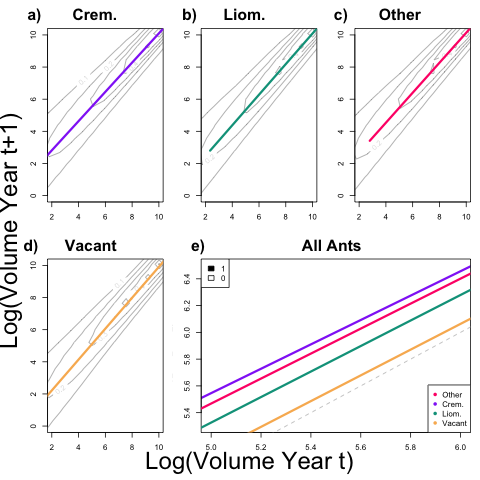
\includegraphics[width=0.95\linewidth]{grow_contour_lines_color.png}
%	\caption{asdasdf}
%	\label{fig:growth}
%\end{figure}
Plants tended by other ants experiened positive growth rates across all sizes, with the highest chances of shrinking occurring at the largest sizes \cite{fig:growth}a.
They experienced significantly higher growth than vacant plants ($p = 2.2 \times 10^{-16}$), and similar mean growth to \textit{L. apiculatum} tended plants ($p = 0.9135$) and \textit{C. opuntiae} tended plants ($p = 0.4864$).  
Plants tended by \textit{C. opuntiae} ants experienced positive growth rates across all sizes, with the highest chances of shrinking occurring at the largest sizes \cite{fig:growth}b.
They experienced significantly higher mean growth than vacant plants ($p = 4.88 \times 10^{-14}$).
Plants tended by \textit{L. apiculatum} experienced positive growth rates across all sizes, with the highest chances of shrinking occurring at the largest sizes \cite{fig:growth}c.
Vacant plants experienced the lowest observed growth, except at the largest sizes where they are less likely to shrink than tended plants \cite{fig:growth}d. 

%% Survival Model
%\begin{figure}[h]
%	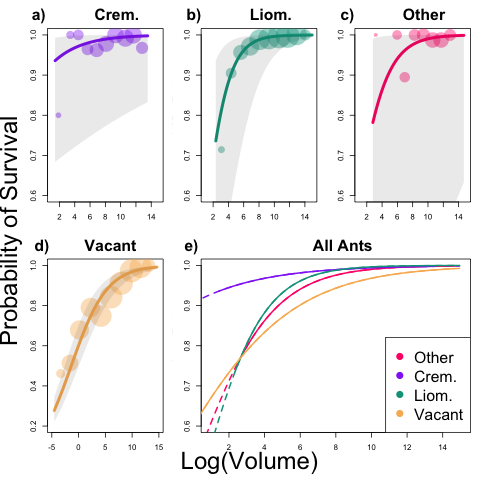
\includegraphics[width=0.95\linewidth]{surv_panels.png}
%	\caption{asdasdf}
%	\label{fig:surv}
%\end{figure}
Plants tended by \textit{C. opuntiae} ants experienced significantly higher mean survival rates than \textit{L. apiculatum} tended plants ($p = 2.908 \times 10^{-14}$), plants tended by other ants ($p = 4.488 \times 10^{-14}$), and vacant plants ($p = 2.2 \times 10^{-16}$) \cite{fig:surv}. 
These \textit{C. opuntiae} plants have the highest mean survival at small sizes before reaching a mean survival rate of about 100\% when medium to large.
Plants tended by \textit{L. apiculatum} experienced similar mean survival rates to plants tended by other ants and vacant plants.
\textit{L. apiculatum} tended plants and other tended plants reached a mean survival rate of nearly 100\% by medium sizes, with other tended plants reaching this rate slower. 
Vacant plants never reach mean survival rates of 100\%. 

%% Flowers Model
There is a clear size effect on the number of flowers produced. 
The mean number of flowers produced by a plant remains at 0 until the plant reachesmedium sizes after which the mean number of flower produced increases eponentially to about 40 at large sizes.


%% Viability Model
%\begin{figure}[h]
%	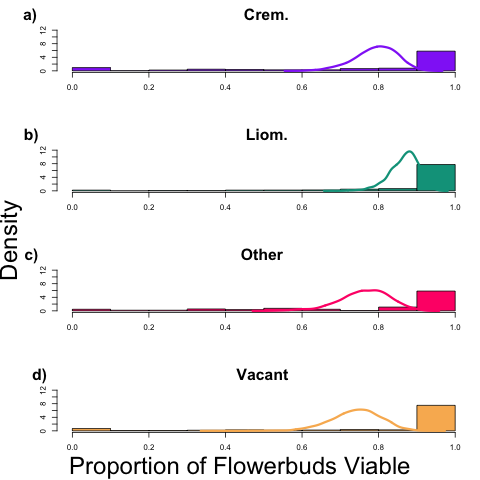
\includegraphics[width=0.95\linewidth]{Viability.png}
%	\caption{asdasdf}
%	\label{fig:comp-samp}
%\end{figure}
Plants tended by \textit{L. apiculatum} ants experienced the highest viability rates, significantly higher than \textit{C. opuntiae} tended plants ($p = 2.2 \times 10^{-16}$), other tended plants ($p = 2.2 \times 10^{-16}$), and vacant plants ($p = 2.2 \times 10^{-16}$).
The mean viability rate of \textit{L. apiculatum} tended plants was 84.888\%.
Plants tended by \textit{C. opuntiae} ants experienced significantly higher viability rates than vacant plants ($p = 2.2 \times 10^{-16}$), but not than other tended plants ($p = 0.1168$).
The mean viability rate of \textit{C. opuntiae} plants was 75.934\%.
Plants tended by other ants also experienced significantly higher viability rates than vacant plants ($p = 2.2 \times 10^{-16}$).
The mean viability rate of other tended plants was 76.367\%.
The mean viability rate of vacant plants was 70.442\%.

%% Reproduction Model
The probability of a plant reproducing in a given year is highly size dependent. 
The mean probability of reproducing remains at about 0\% until the plant reaches a medium size, after which the mean probability of reproducing increases steadily before reaching about 100\% at large sizes. 

%% Seeds Produced
The mean number of seeds produced by \textit{C. opuntiae} tended plants is significantly lower than the mean number of seeds produced by \textit{L. apiculatum} plants ($p = 2.2 \times 10^{-16}$) and vacant plants ($p = 2.2 \times 10^{-16}$). 
\textit{C. opuntiae} tended plants produce a mean of 2.561 seeds per flower. 
The mean number of seeds produced by \textit{L. apiculatum} tended plants is slightly higher than the mean number produced by vacant plants ($p = 0.02521$). 
\textit{L. apiculatum} tended plants produce a mean of 3.563 seeds per flower. 
Vacant plants produce a mean of 3.435 seeds per flower. 

%% Precensus Survival
The mean pre-census seed survival rate is 16.99\% with 90\% of model iterations landing between 1.13\% and 40.72\%. 

%% Germination
Seeds have a significantly higher probability of germinating in year one than in year two ($p = 2.2 \times 10^{-16}$).
Seeds in year one have a mean germination rate of 0.578\% and seeds in year two have a mean germination rate of 0.221\%. 

%% Recruit size distribution
The mean size of new recruits is -1.88 log($cm^3$) with 90\% of new recruits falling between the sizes of -2.12 log($cm^3$) and -1.64 log($cm^3$).

%% Ant Transition Rates
% previously vacant
Plants that were previously vacant will most likely remain vacant until large. 
These plants have significantly higher probabilities of being vacant rather than becoming tended  by \textit{C. opuntiae}, \textit{L. apiculatum}, or other ants (respectively, $p = 2.2 \times 10^{-16}$, $p = 2.2 \times 10^{-16}$, and $p = 2.2 \times 10^{-16}$).
The probability of previously vacant plants becoming tended by \textit{L. apiculatum} ants is significantly higher than the probabilities of becoming tended by \textit{C. opuntiae} or other ants (respecitvely, $p = 3.83 \times 10^{-14}$, $p = 2.2 \times 10^{-16}$).
The probability of previously vacant plants becoming tended by other ants is significantly lower than the probability of becoming tended by \textit{C. opuntiae} ($p = 0.00227$).

% previously crem
Plants that were previously tended by \textit{C. opuntiae} will most likely remain vacant until large. 
These plants have significantly higher probabilities of becoming vacant rather than remaining tended by \textit{C. opuntiae} or becoming tended by \textit{L. apiculatum} or other ants (repsectively, $p = 2.2 \times 10^{-16}$, $p = 2.2 \times 10^{-16}$, $p = 2.2 \times 10^{-16}$ ).
The probability of these plants remaining tended by \textit{C. opuntiae} ants is significantly higher than the probability of becoming tended by \textit{L. apiculatum} or other ants (respectively, $p = 2.2 \times 10^{-16}$, $p = 3.797 \times 10^{-9}$).
The probability of these plants becoming tended by \textit{L. apiculatum} is significantly higher than the probability of becoming tended by other ants ($p = 3.797 \times 10^{-9}$).

% previously liom
Plants that were previously tended by \textit{L. apiculatum} ants will most likely remain vacant until large. 
These plants have significantly higher probabilities of becoming vacant than remaining tended by \textit{L. apiculatum} or becoming tended by \textit{C. opuntiae} or other ants (respectively, $p = 2.2 \times 10^{-16}$, $p = 2.2 \times 10^{-16}$, and $p = 2.2 \times 10^{-16}$).
These plants have significantly higher probabilities of remaining tended by \textit{L. apiculatum} ants than becoming tended by  \textit{C. opuntiae} or other ants (respectively, $p = 2.2 \times 10^{-16}$, $p = 2.2 \times 10^{-16}$).
The probability of these plants becoming tended by \textit{C. opuntiae} ants is significantly higher than the probability of them becoming tended by other ants ($p = 0.007925$).

% previously other
Plants that were previously tended by other ants will most likely remain vacant until they are large. 
These plants have significantly higher probabilities of becoming vacant rather than remaining tended by other ants or becoming tended by \textit{C. opuntiae} or \textit{L. apiculatum} ants (respectively, $p = 2.2 \times 10^{-16}$, $p = 2.2 \times 10^{-16}$, $p = 2.2 \times 10^{-16}$).
The probability of these plants becoming tended by \textit{L. apiculatum} ants is significantly higher than the probability of remaining tended by other ants or becomnig tended by \textit{C. opuntiae} (respectively, $p = 6.309 \times 10^{-12}$, $p = 6.256 \times 10^{-13}$).
The probability of these plants remaining tended by other ants is not higher than the probability of becoming tended by \textit{C. opuntiae} ants ($p = 0.954$). 

%% All cases/trends
In all plants ,the most likely scenario is vacancy.
In most cases, the second most likely next ant partner is \textit{L. apiculatum} with the exception of plants which were previously tended by \textit{C. opuntiae} who are second most likely to retain \textit{C. opuntiae} as their partners in successive years.
The only case where two next partners do not have statistically significantly different probabilities is when previously other tended plants either remain tended by other ants or become tended by \textit{C. opuntiae}. 

\subsection*{Deterministic IPM}

\subsection*{Stochastic IPM}


\section*{Discussion}


\section*{Acknowledgments}

%%%%%%%%%%%%%%%%%%%%%
% Statement of Authorship
%%%%%%%%%%%%%%%%%%%%%
% This section should also be commented out while your MS is undergoing
% double-blind review. The specifics should of course be adapted to
% your paper, but the paragraph below gives some hints of possible
% contributions.

\section*{Data and Code Availability}

\section*{Appendix A: Additional Methods and Parameters}

% In most cases, authors should typeset supplementary material in a separate,
% author-supplied PDF. For author-supplied PDFs, please consult the
% AmNat_supp_template.tex document, available from
% https://www.journals.uchicago.edu/journals/an/instruct 
%
% By contrast, the Appendix instructions below apply to cases in which
% a brief appendix is to appear in print after the main body of the article.
% That notably includes descriptions of methods, tables defining parameters,
% and other material necessary for reproducing the MS's results.
%
% Please reset counters for the appendix (thus normally figure A1, 
% figure A2, table A1, etc.).
%
% Most AmNat articles have no more than one print appendix. If your article
% has more than one, counters for each appendix should match the letter of
% that appendix. For example, tables in Appendix B should be numbered table B1, % table C2, etc. This applies to tables, equations, and figures.
%
% It's better not to use the \appendix command, because we have some
% formatting peculiarities that \appendix conflicts with.

\renewcommand{\theequation}{A\arabic{equation}}
% redefine the command that creates the equation number.
\renewcommand{\thetable}{A\arabic{table}}
\setcounter{equation}{0}  % reset counter 
\setcounter{figure}{0}
\setcounter{table}{0}

%%%%%%%%%%%%%%%%%%%%%
% Bibliography
%%%%%%%%%%%%%%%%%%%%%
% You can either type your references following the examples below, or
% compile your BiBTeX database and paste the contents of your .bbl file
% here. The amnatnat.bst style file should work for this---but please
% let us know if you run into any hitches with it!
%
% If you upload a .bib file with your submission, please upload the .bbl
% file as well; this will be required for typesetting.
%
% The list below includes sample journal articles, book chapters, and
% Dryad references.
\bibliographystyle{apalike}
\bibliography{References.bib}


\newpage{}

\section*{Tables}
\renewcommand{\thetable}{\arabic{table}}
\setcounter{table}{0}

\renewcommand{\thetable}{\arabic{table}}
\setcounter{table}{0}

% I am creating a table here to include all parameter estimations and descriptions
  \begin{table}[]
  \begin{tabular}{l|l|l}
    \textbf{Parameter} & \textbf{Median ($95\%$ CI)} & \textbf{Prior Distribution} \\
    \hline
    %% Growth Parameters
    growth xi intercept vacant $\beta_{01}^g$ & $-5.210899 (-5.686865, -5.491787)$ & sDE\\
    growth xi intercept other $\beta_{02}^g$ & $-5.8288 (-5.956217, 1.766021) $&asdf \\
    growth xi intercept \textit{C. opuntiae} $\beta_{03}^g$ & $-4.529523 (-6.0770390, 0.1222112)$ & asdf\\
    growth xi intercept \textit{L. apiculatum} $\beta_{04}^g$ & $-5.106802 (-5.4499944, 0.5453901)$ & asdf\\
    growth xi size dependent vacant $\beta_{11}^g$ & asdf&asdf \\
    growth xi size dependent other $\beta_{12}^g$ & asdf&asdf \\
    growth xi size dependent \textit{C. opuntiae} $\beta_{13}^g$ & asdf&asdf \\
    growth xi size dependent \textit{L. apiculatum} $\beta_{14}^g$ &sadf &asdf \\
    growth omega intercept $\omega_0^g$ & & \\
    growth omega size dependent $\omega_1^g$ & & \\
    growth alpha intercept $\alpha_0^g$ & & \\
    growth alpha size dependent $\alpha_1^g$ & & \\
    \hline
    %% Germination Parameters
    1-year germination intercept $\alpha^{\gamma_1}$ & & \\
    2-year germination intercept $\alpha^{\gamma_2}$ & & \\
    \hline
    %% Survival Parameters
    survival intercept vacant $\beta_{01}^s$ & & \\
    survival intercept other $\beta_{02}^s$ & & \\
    survival intercept \textit{C.opuntiae} $\beta_{03}^s$ & & \\
    survival intercept \textit{L. apiculatum} $\beta_{04}^s$ & & \\
    survival size dependent vacant $\beta_{11}^s$ & & \\
    survival size dependent other $\beta_{12}^s$ & & \\
    survival size dependent \textit{C. opuntiae} $\beta_{13}^s$ & & \\
    survival size dependent \textit{L. apiculatum} $\beta_{14}^s$ & & \\
    \hline
    %% Probability of Flowering Parameters
    flowering intercept $\beta_0^f$ & & \\
    flowering size dependent $\beta_1^f$ & & \\
    \hline
    %% Floral Viability Parameters
    viability intercept vacant $\beta_01^v$ & & \\
    viability intercept other $\beta02^v$ & & \\
    viability intercept \textit{C. opuntiae} $\beta_03^v$ & & \\
    viability intercept \textit{L. apiculatum} $\beta_04^v$ & & 
  \end{tabular}
  \end{table}

\section*{Figure legends}


%%%%%%%%%%%%%%%%%%%%
 Videos
%%%%%%%%%%%%%%%%%%%%
 If you have videos, journal style for them is generally similar to that for
 figures. 

%%%% Include the text below if you have videos



%%%% Include the above if you have videos


\end{document}
